% ============================================================
% DRAFT of the implementation paper (Prompt 15), T21 Version A.
% Draft text written with an AI assistant from the verified evidence; to be
% reviewed and revised by the student (see the AI Assistance Disclosure).
% Same layout as the mid-semester review (article, two-column, natbib).
% Red [WRITE: ...] boxes = notes for YOU to turn into your own sentences.
% Orange [TO VERIFY: ...] = facts to check before submission.
% Every number below comes from results/results.csv (run of 17 Nov 2026).
% Tables in tables/ are written by src/analyse_a.py: never retype numbers.
% Write the Abstract LAST. Delete all \writeit and \tv before submission.
% ============================================================
\documentclass[10pt,twocolumn]{article}

\usepackage[a4paper,margin=1.9cm,columnsep=0.6cm]{geometry}
\usepackage{times}
\usepackage{amsmath}
\usepackage{graphicx}
\usepackage{tikz}
\usetikzlibrary{arrows.meta,positioning}
\usepackage{booktabs}
\usepackage{caption}
\usepackage{xurl}
\usepackage[colorlinks=true,linkcolor=blue!50!black,citecolor=blue!50!black,urlcolor=blue!50!black]{hyperref}
\usepackage[round]{natbib}
\usepackage{fancyhdr}
\usepackage{titlesec}
\usepackage{enumitem}
\usepackage{xcolor}
\usepackage{abstract}

\setlength{\parindent}{0pt}
\setlength{\parskip}{4pt}
\titleformat{\section}{\normalfont\large\bfseries}{\thesection}{0.6em}{}
\titleformat{\subsection}{\normalfont\normalsize\bfseries}{\thesubsection}{0.6em}{}
\titlespacing*{\section}{0pt}{10pt}{4pt}
\titlespacing*{\subsection}{0pt}{8pt}{3pt}
\pagestyle{fancy}
\fancyhf{}
\fancyhead[L]{\small Verifying LLM Citations: Rules, Strings or Databases?}
\fancyhead[R]{\small AITR Implementation Paper}
\fancyfoot[C]{\small\thepage}
\renewcommand{\headrulewidth}{0.4pt}
\captionsetup{font=small,labelfont=bf}

\newcommand{\writeit}[1]{\textcolor{red!70!black}{\textbf{[WRITE:} #1\textbf{]}}}
\newcommand{\tv}[1]{\textcolor{orange!80!black}{\textbf{[TO VERIFY:} #1\textbf{]}}}

\title{\vspace{-1.2cm}\textbf{Rules, Strings or Databases? Checking Fabricated Citations from Two Open-Weight Language Models}}
\author{Vaibhav Sharma \\ \small Roll No. MSE2026010 \\ \small Department of Software and Automation \\ \small Indian Institute of Information Technology Allahabad (IIIT-A)}
\date{}

\begin{document}
\twocolumn[
  \begin{@twocolumnfalse}
    \maketitle
    \begin{abstract}
Language models often produce references that look plausible but do not exist, and studies that measure this rely on some way of checking each citation. We compare three such checkers on the same output: a rule baseline that inspects the citation string for missing or malformed fields (B0), a string-only logistic regression detector that never queries a database (B1), and a matcher that searches CrossRef and OpenAlex and resolves DOIs (B2). Two open-weight models, Qwen2.5-7B-Instruct and Mistral-7B-Instruct-v0.3, were each asked for ten references on six computer science topics under a protocol frozen before the main run. Of the 108 citations produced, 103 (95.4\%) were labelled fabricated and none was fully correct. Ranked by AUC, database matching (0.817) was ahead of the string detector (0.672) and the rule baseline (0.415); the rule baseline caught only 2.9\% of fabricated citations, because invented references were complete and well formed. Database matching missed 15 fabricated citations whose generic titles were close to real papers by other authors, and cost 5.2 seconds and 3.7 API calls per citation. The reference labels were produced with AI assistance and partly from the same databases used by B2, so B2's scores are an upper bound. All code, data and decisions are released.
    \end{abstract}
    \vspace{0.5em}
  \end{@twocolumnfalse}
]

% ------------------------------------------------------------
\section{Introduction}
Large language models are now used to draft literature reviews, related work sections and reading lists. A known weakness is that they produce references that are partly or wholly invented: author lists, titles, venues and DOIs that look correct but point to no real publication \citep{alkaissi2023,walters2023}. This is one instance of the broader hallucination problem in text generation \citep{ji2023}, but it has a direct cost in research, since an invented citation can enter a manuscript and survive review.

Most work on this problem reports how often models fabricate. To do so, every audit needs a way to decide whether a given citation exists, and the choice of checker shapes the reported rate. Some checks look only at the citation string, some train a classifier on string features \citep{naser2026}, and some look the citation up in scholarly databases \citep{rao2026}. In the literature reviewed for this work, these families are rarely compared on the same citations, and their cost is seldom reported.

This paper compares three checkers on citations produced by two open-weight 7B models under a protocol that was frozen before the main run. We ask two questions:
\begin{itemize}[leftmargin=*,itemsep=1pt,topsep=2pt]
\item \textbf{RQ1.} How do a rule baseline (B0), a string-only detector (B1) and database matching (B2) compare in accuracy and cost against reference labels?
\item \textbf{RQ2.} Does a string-only detector trained on one model's citations keep its performance on another model's citations?
\end{itemize}
The contributions are modest and empirical: (i) a side-by-side comparison of the three checker families on the same citations, including cost; (ii) a failure analysis of database matching, which shows how generic titles defeat title similarity; (iii) two negative results, for rule checks and for detector transfer, reported as observed; and (iv) a public pipeline with every protocol decision logged. The study does not propose a new detection method.

% ------------------------------------------------------------
\section{Related Work}
\subsection{How often models fabricate references}
Early reports documented invented references in ChatGPT output in scientific writing \citep{alkaissi2023} and measured fabrication and bibliographic errors across many generated citations \citep{walters2023}. Later studies varied the setting: topic familiarity and prompt specificity \citep{linardon2025}, citation reliability across disciplines \citep{mugaanyi2024}, a reference hallucination score for medical chatbots \citep{aljamaan2024}, and large-scale analyses of citation validity \citep{xu2026} and of citation bias in model output \citep{algaba2024}. The legal domain has received particular attention, with profiles of legal hallucinations \citep{dahl2024}, evaluations of commercial legal research tools \citep{magesh2025} and a citation reliability benchmark \citep{chen2026}. Problems with citations in AI search products have also been reported \citep{jazwinska2025}. Taken together, these studies show that the measured rate depends strongly on model, domain, prompt and the way citations are checked. Numbers from these studies are not repeated here, because they were not re-verified for this work.

\subsection{Ways to check a citation}
Three families of checks can be distinguished. \emph{Format checks} inspect the citation string for missing or malformed fields, such as a missing DOI or an impossible year. \emph{String-only detectors} learn to separate fabricated from real citations using features of the string alone; \citet{naser2026} audits reference fabrication across models and proposes methods to detect such ``phantom citations''. \emph{Database lookup} searches scholarly indexes and compares the best match with the citation; \citet{rao2026} study detecting and correcting reference hallucinations in commercial models and deep research agents. Methods that check consistency across several samples of the same model, such as SelfCheckGPT \citep{manakul2023}, form a fourth family that needs no external source; they are not studied here. Retrieval-augmented generation \citep{lewis2020} reduces the problem at generation time rather than checking afterwards. In this study B0 is a format check, B1 a string-only detector and B2 a database lookup.

\subsection{Gap}
In the literature reviewed for this work, we did not find a study that compares all three checker families on the same open-weight model output, against reference labels, while reporting cost per citation. This study fills that gap at a small scale.

% ------------------------------------------------------------
\section{Method}
\begin{figure}[t]
\centering
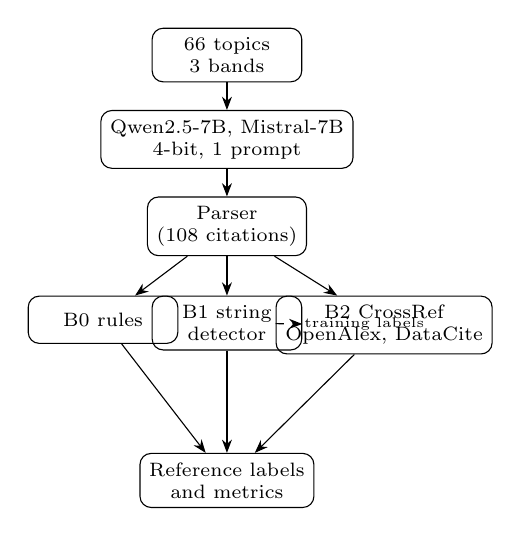
\begin{tikzpicture}[node distance=0.35cm, every node/.style={draw, rounded corners, font=\scriptsize, align=center, minimum width=1.9cm, minimum height=0.6cm}, >=Stealth]
\node (t) {66 topics\\3 bands};
\node (g) [below=of t] {Qwen2.5-7B, Mistral-7B\\4-bit, 1 prompt};
\node (p) [below=of g] {Parser\\(108 citations)};
\node (b0) [below left=0.5cm and -0.4cm of p] {B0 rules};
\node (b1) [below=0.5cm of p] {B1 string\\detector};
\node (b2) [below right=0.5cm and -0.4cm of p] {B2 CrossRef\\OpenAlex, DataCite};
\node (r) [below=1.3cm of b1] {Reference labels\\and metrics};
\draw[->] (t) -- (g); \draw[->] (g) -- (p);
\draw[->] (p) -- (b0); \draw[->] (p) -- (b1); \draw[->] (p) -- (b2);
\draw[->] (b0) -- (r); \draw[->] (b1) -- (r); \draw[->] (b2) -- (r);
\draw[->, dashed] (b2) -- node[draw=none, right, font=\tiny]{training labels} (b1);
\end{tikzpicture}
\caption{Pipeline. B1 is trained on B2 labels and evaluated against reference labels.}
\label{fig:pipeline}
\end{figure}

Figure~\ref{fig:pipeline} summarises the pipeline. All settings were written in a configuration file that was frozen, together with pinned model revisions, before the main run; every change before freezing is logged in the project repository.

\subsection{Topics and generation}
We started from 90 candidate computer science topics. For each, we counted the works returned by an OpenAlex keyword search \citep{priem2022openalex} and split the topics into three prominence bands (terciles). From each band, two topics were set aside as pilot topics, used only to choose thresholds. Because of time limits, the main run used two further topics per band, six in total, drawn with a fixed seed: approximate computing and software defined networking (high), code review automation and distributed consensus algorithms (medium), and dark pattern detection in user interfaces and technical debt in machine learning (low). The bands serve only to spread the topics; prominence is not analysed, since keyword search counts are a rough measure.

Two instruction-tuned open-weight models were used, Qwen2.5-7B-Instruct and Mistral-7B-Instruct-v0.3, loaded in 4-bit NF4 format with their Hugging Face revisions pinned. Each received one user message asking for ten peer-reviewed references on the topic, with authors, year, title, venue and DOI, numbered from 1 to 10. Sampling used temperature 0.7, top-p 0.9, at most 1,024 new tokens and seed 11.

\subsection{Parsing}
Answers were split into citations by a deterministic regular-expression parser; no model was used, so parsing cannot add or remove citations. Only numbered lines start a new citation, and a separate reader handles answers written as labelled fields (``Title:'', ``Year:'', ``DOI:''). Both rules were added after the pilot showed that indented sub-fields had been split into separate citations, before any main-run output existed.

\subsection{The three checkers}
\textbf{B0, rule baseline.} Six red flags are computed from the citation string: no DOI, malformed DOI, no year, a year after 2026 or before 1950, no authors, and a title shorter than four words. A citation is called fabricated if it raises at least one flag; this setting was chosen on the pilot, where two flags caught nothing.

\textbf{B1, string-only detector.} A logistic regression (balanced class weights, $C=1$) uses 16 features of the string, among them its length, number of title words and authors, presence of ``et al.'', presence and prefix of a DOI, DOI suffix length, presence and age of the year, page and volume patterns, a venue word, a colon in the title, the share of capital letters, a URL and the number of digits. No feature may come from a database lookup; the code refuses to run if one does. Because only the reference set is labelled, B1 is trained on B2's labels and evaluated against the reference labels, with out-of-fold predictions from five folds grouped by topic, so that no topic appears in its own training fold.

\textbf{B2, database matching.} Each citation's title (with its first author) is searched in CrossRef, and its title in OpenAlex. The best candidate is the one with the highest title similarity (token sort ratio after normalisation). A citation scoring below $t=0.85$ is called fabricated; $t$ was chosen on 57 labelled pilot citations. Otherwise, B2 checks the first author's surname, the year (within one), DOI equality and DOI resolution, first in CrossRef and then in DataCite, which holds arXiv and Zenodo DOIs. A failed check gives ``metadata error'', otherwise ``exists''. CrossRef requests were limited to three per second.

\subsection{Reference labels}
Each citation received one of four labels following a written rubric: \emph{exists}, \emph{metadata error} (a real work cited with a wrong author, year or DOI, or an altered title), \emph{fabricated}, or \emph{unresolvable}. A citation counts as the same work as a real paper only if the title is near-identical and the first author or the year matches; for generic titles such as ``X: A Survey'', the first author must match. The labels were produced with an AI assistant, using database and web lookups and its own knowledge, and were reviewed by the author. Most labels relied in part on the same CrossRef and OpenAlex results that B2 uses. The reference labels are therefore not independent of B2, and B2's scores below should be read as an upper bound.

% ------------------------------------------------------------
\section{Experimental Setup}
The pilot (12 answers, 89 citations) ran on a Google Colab T4 GPU. The main run ran on Kaggle with two T4 GPUs, one model per GPU in parallel, using Python 3.13.16, PyTorch 2.11.0 and Transformers 5.20.2; generation, parsing and database matching took 20.4 minutes in total. The protocol was frozen on 17 November 2026 at 11:35 UTC, before generation started.

For RQ1 we report precision, recall and F1 for the class ``fabricated'', each with a 95\% Wilson interval \citep{wilson1927}, specificity on the non-fabricated citations, and AUC from each checker's score (the number of B0 flags, B1's probability, and one minus B2's best title similarity). Differences in F1 are given with a paired bootstrap over topics (1,000 resamples, seed 2026). Because almost all citations turned out to be fabricated, we also report a trivial rule that calls every citation fabricated. Cost is the mean time and number of API calls per citation. For RQ2, B1 is trained on all citations of one model and tested on the other, and compared with its out-of-fold AUC within the test model; this comparison is scored against B2's labels, since the reference set is too small to split by model. All checkers saw the same citations and the same labels, and no threshold was changed after the main run.

% ------------------------------------------------------------
\section{Results}
\subsection{Corpus}
The two models gave 12 answers. Seven answers reached the 1,024-token limit (three from Qwen, four from Mistral), so their last reference was cut short or missing. The parser extracted 108 citations, 58 from Qwen and 50 from Mistral, and all were parsed completely. Seven citations repeated an earlier one in the same answer; they were kept, since they are part of what the models produced.

\begin{table}[t]
\centering
\small
\setlength{\tabcolsep}{3pt}
\caption{Fabrication rate under two definitions (B2 labels).}
\label{tab:fr}
\begin{tabular}{llllll}
\toprule
model & fr\_exist & CI & fr\_broad & CI broad & n \\
\midrule
Qwen2.5-7B & 0.879 & 0.77 to 0.94 & 1.000 & 0.94 to 1.00 & 58 \\
Mistral-7B & 0.780 & 0.65 to 0.87 & 1.000 & 0.93 to 1.00 & 50 \\
\bottomrule
\end{tabular}
\end{table}

\subsection{How many citations were fabricated}
Against the reference labels, 103 of the 108 citations (95.4\%) were fabricated. The other five were real works cited with errors: a 2014 survey of software defined networking cited with a shortened title and the second author listed first, the 1985 impossibility result for distributed consensus with a DOI that does not resolve, a well-known circuit design textbook with an altered title, and two papers on multi-agent consensus with altered titles and a wrong year, venue or DOI. No citation was fully correct. The rate was 0.948 for Qwen (95\% interval 0.86 to 0.98) and 0.960 for Mistral (0.87 to 0.99); the intervals overlap almost completely, so no difference between the models can be claimed. B2 alone gives lower rates (Table~\ref{tab:fr}), 0.879 and 0.780, because it accepts some fabricated citations as metadata errors (Section~\ref{sec:fail}).

\begin{table*}[t]
\centering
\small
\setlength{\tabcolsep}{3pt}
\caption{Verifier comparison against the reference labels (class: fabricated; Wilson 95\% CIs).}
\label{tab:verifiers}
\begin{tabular}{llllllllll}
\toprule
verifier & precision & P 95\% CI & recall & R 95\% CI & f1 & specificity & tp & fp & fn \\
\midrule
B0 rules & 0.750 & 0.30 to 0.95 & 0.029 & 0.01 to 0.08 & 0.056 & 0.800 & 3 & 1 & 100 \\
B1 string detector & 0.968 & 0.91 to 0.99 & 0.893 & 0.82 to 0.94 & 0.929 & 0.400 & 92 & 3 & 11 \\
B2 database & 0.978 & 0.92 to 0.99 & 0.854 & 0.77 to 0.91 & 0.912 & 0.600 & 88 & 2 & 15 \\
B1 without DOI features (ablation) & 0.969 & 0.91 to 0.99 & 0.913 & 0.84 to 0.95 & 0.940 & 0.400 & 94 & 3 & 9 \\
Trivial: all fabricated & 0.954 & 0.90 to 0.98 & 1.000 & 0.96 to 1.00 & 0.976 & 0.000 & 103 & 5 & 0 \\
\bottomrule
\end{tabular}
\end{table*}

\subsection{RQ1: comparing the checkers}
Table~\ref{tab:verifiers} shows the comparison. The trivial rule, which calls everything fabricated, has the highest F1 (0.976) while recognising none of the five real works. With 95\% of citations fabricated, F1 for the fabricated class therefore cannot rank the checkers, and we rely on AUC and specificity, while noting that specificity rests on only five cases.

By AUC, B2 ranked first (0.817), followed by B1 (0.672) and B0 (0.415, below chance). B0 flagged only 4 of 108 citations and caught 3 of the 103 fabricated ones (recall 0.029, interval 0.01 to 0.08). B2 and B1 both caught most fabricated citations (recall 0.854 and 0.893). The F1 difference between B2 and B0 was 0.856 (bootstrap interval 0.771 to 0.933), while the difference between B2 and B1 was $-0.017$ (interval $-0.118$ to $0.098$), so B2 and B1 cannot be separated by F1 on these data. Removing B1's three DOI features did not reduce its performance (F1 0.940), which suggests that B1 did not depend on the presence of a DOI.

\begin{figure}[t]
\centering
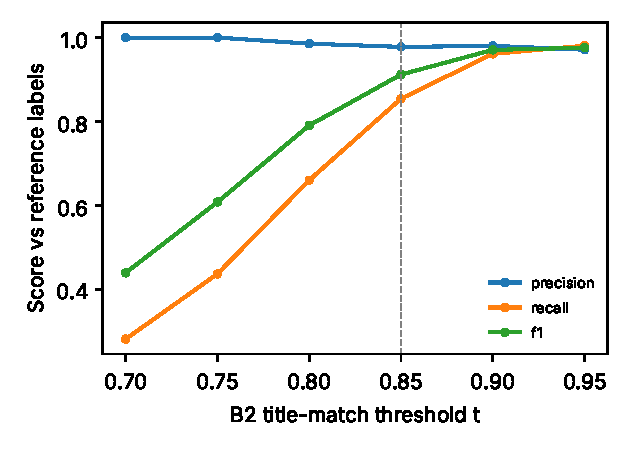
\includegraphics[width=\linewidth]{figures/f2_b2_sensitivity.pdf}
\caption{B2 precision, recall and F1 against the reference labels for title thresholds 0.70 to 0.95 (main run). Dashed line: frozen threshold 0.85.}
\label{fig:sens}
\end{figure}

\subsection{Where database matching fails}\label{sec:fail}
B2 disagreed with the reference labels on 17 citations. In 15 cases, an invented title with generic wording scored at or above 0.85 against a real paper by other authors; for example, ``Technical Debt in Machine Learning: A Survey'' was matched to the real ``Technical Debt in Machine Learning Systems''. B2 then checked the authors and DOI, found them wrong, and reported a metadata error instead of a fabrication. In the other two cases, real papers cited with altered titles scored 0.75 and 0.80 and were called fabricated. Figure~\ref{fig:sens} shows that, on these data, a higher threshold would have caught more of the fabricated citations. Because the threshold was fixed on the pilot before the main run, this is reported as an observation only and was not used to change B2.

\begin{table}[t]
\centering
\small
\setlength{\tabcolsep}{3pt}
\caption{Cost per citation (B1 time includes training within cross-validation).}
\label{tab:cost}
\begin{tabular}{lll}
\toprule
verifier & sec\_per\_cit & api\_per\_cit \\
\midrule
B0 rules & 0.000 & 0.000 \\
B1 string detector & 0.001 & 0.000 \\
B2 database & 5.181 & 3.685 \\
\bottomrule
\end{tabular}
\end{table}

\subsection{Cost}
Table~\ref{tab:cost} reports cost. B2 needed 5.18 seconds and 3.69 API calls per citation, partly because CrossRef requests were limited to three per second. B0 and B1 needed less than a millisecond and no network access, even though B1's time includes training within cross-validation.

\begin{table*}[t]
\centering
\small
\setlength{\tabcolsep}{3pt}
\caption{Transfer of the string-only detector B1 (AUC against B2 labels; 95\% topic bootstrap CI of the drop).}
\label{tab:transfer}
\begin{tabular}{llllllll}
\toprule
test\_model & train\_model & auc\_within & auc\_transfer & drop & ci\_lo & ci\_hi & n \\
\midrule
Qwen2.5-7B & Mistral-7B & 0.471 & 0.695 & -0.224 & -0.518 & -0.020 & 58 \\
Mistral-7B & Qwen2.5-7B & 0.371 & 0.408 & -0.037 & -0.241 & 0.262 & 50 \\
\bottomrule
\end{tabular}
\end{table*}

\begin{figure}[t]
\centering
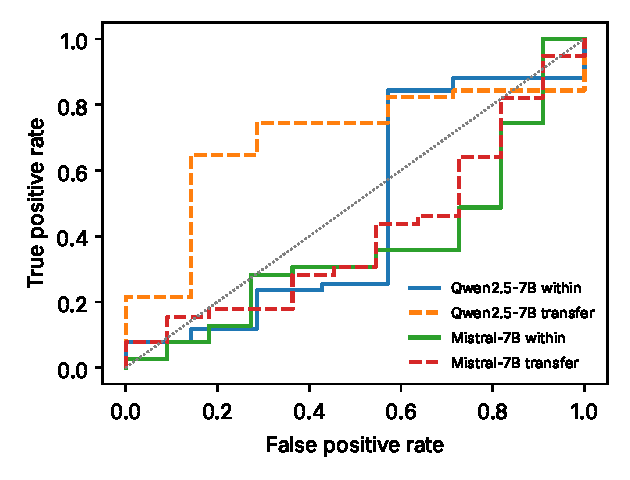
\includegraphics[width=\linewidth]{figures/f1_roc_transfer.pdf}
\caption{ROC curves of B1 within each model and after training on the other model (scored against B2 labels).}
\label{fig:roc}
\end{figure}
\subsection{RQ2: does the string detector transfer?}
Table~\ref{tab:transfer} and Figure~\ref{fig:roc} report B1 within each model and after training on the other. Within one model, B1's AUC was below chance (0.471 for Qwen, 0.371 for Mistral). Trained on the other model, it reached 0.695 on Qwen and 0.408 on Mistral. B1 was trained on B2's labels, which contain only 18 non-fabricated citations spread over six topics, so each within-model fold held very few of them. Since the within-model baseline did not work, the planned test of a drop in AUC between models cannot be applied meaningfully, and RQ2 remains unanswered by this study.

% ------------------------------------------------------------
\section{Discussion}
The clearest result is the failure of rule checks. Both models produced citations that were complete and well formed: they had authors, years, venues and, in most cases, DOIs. Checks for missing or malformed fields cannot see invention of this kind, and for these models a rule baseline is not a useful filter. This fits the pattern of plausible-looking fabricated references reported in earlier audits \citep{walters2023}.

Database matching ranked best by AUC, but its main error mode deserves attention. Titles such as ``X: A Survey'' are close in wording to many real papers, and a title similarity score cannot tell ``a paper with these words exists'' from ``this paper exists''. In our data, this caused 15 of B2's 17 errors. A possible remedy is to require an author match when a title is generic; we have not tested it.

Whether a string-only detector can approach database matching remains open. B1's AUC was lower than B2's, but its F1 was similar, and with five non-fabricated citations neither specificity nor the difference between them can be estimated reliably. B1 was also trained on B2's labels, so it could at best learn B2's view of the data.

For someone checking model-generated references, the practical reading of these results, within the limits of this study, is that format checks give false reassurance, that database lookup is the most informative of the three but needs care with generic titles, and that its cost of a few seconds per citation is acceptable for manual review of a reference list.

\section{Limitations}
First, the reference labels were produced with AI assistance and partly from the same databases as B2; B2's results are therefore an upper bound, and an independent human labelling is needed to confirm them. Second, the sample is small: six topics, 108 citations, only five non-fabricated works, one seed and one run. Third, seven of twelve answers were cut at the token limit. Fourth, only two 7B models in 4-bit format and one prompt were tested; commercial models and agentic search tools, which motivate the wider topic, were not studied. Fifth, the protocol changed before freezing: reproducing an earlier detector was dropped because its data and code were not available, and the main run was reduced to six topics. Finally, the pilot and the main run used different platforms and library versions, although all main-run comparisons share one environment.

\section{Future Work}
Three follow-up experiments would add the most information for their cost. The cheapest is to have a human relabel all 17 citations where B2 disagreed with the reference labels plus 30 random others, using Google Scholar only, and to report agreement with the current labels. The second is to test one isolated change to B2, requiring an author match for generic titles, chosen on the pilot and evaluated on the same 108 citations. The most expensive is a full run over 60 topics with a 2,048-token limit, which would give enough real citations to estimate specificity and to test transfer between models.

\section{Conclusion}
We compared a rule baseline, a string-only detector and database matching on 108 citations produced by two open-weight 7B models. Almost all citations were fabricated, and none was fully correct. Rule checks caught almost none of them, because the fabricated citations were well formed. Database matching ranked best by AUC at a cost of about five seconds per citation, but it was misled by generic titles that resemble real papers. These results come from a small sample with AI-made reference labels, and the pipeline and all decisions are public so that they can be checked and extended.

\section*{AI Assistance Disclosure}
In line with Section 10 of the course brief: the code was written with an AI assistant (Claude, Anthropic) and tested by the author; the author ran the pilot on Google Colab and the main run on Kaggle; the reference labels were produced with the AI assistant and reviewed by the author; and the text of this paper was drafted with the AI assistant from the logged evidence and then reviewed and revised by the author. All AI contributions and the author's checks are recorded in \texttt{ai\_assistance\_log.md}, and all protocol decisions in \texttt{research\_decisions.md}.

\section*{Code and Data Availability}
Code, configuration, model outputs, labels, results and logs are available at \url{https://github.com/VaibhavIITA/Awesome-Benchmarking-citation-fabrication-llms}, in the folder \texttt{implementations/citeverify}. All tables and figures are generated by \texttt{python -m src.analyse\_a} from \texttt{results/} and \texttt{data/}.

\bibliographystyle{plainnat}
\bibliography{refs}

\end{document}
